\chapter{Load Testing}

\section{Test Scenario: List all Games}\label{sec:scenario-list-all-games}
In this scenario, a user logs in to our website, visits the list of games, and then logs out. We constructed tsung script having four phases, each being one minute in duration. The arrival rate in phase one was two users per second. The arrival rate was doubled in each subsequent phases. We ran this script first without having pagination on the list of games which contained more than 15000 entries. This showed us that near the end of phase one (i.e. near the end of the first minute) the mean duration of the requests spiked suddenly to 14 seconds. The duration started decreasing down to about 3.5 seconds at the start of the second phase and remained moderately constant throughout the second and third phase. Finally during the final phase the mean duration again spiked to eight minutes and in some cases ten. This is not unexpected as the number of users is much higher in the final phase. These mean durations were certainly higher than a user would expect. We presumed showing all of the games in the list was causing such long durations. Our presumption was supported when we ran the tsung script again. However, we paginated our games list this time. It showed us a near flat mean duration of fractions of a second all throughout the four phases. Figure~\ref{fig:effect-of-pagination-on-game-list} shows the comparison of the mean duration of requests for the current scenario with and without pagination.

\begin{figure}
\centering
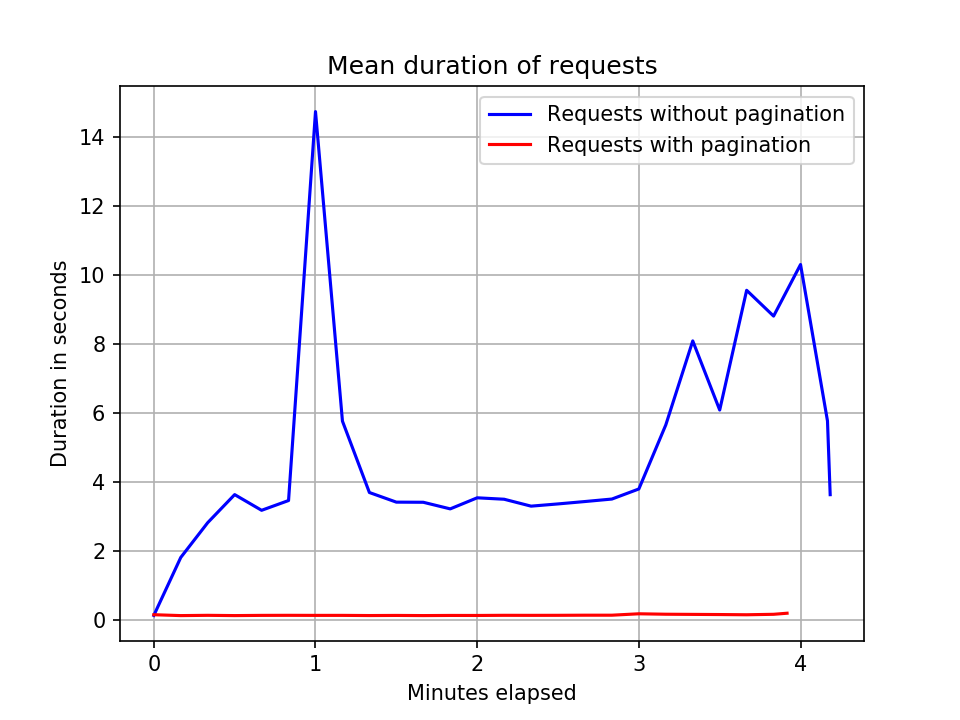
\includegraphics{images/tsung/request_mean_game_index_pagination.png}
\caption{Mean duration of pages before and after pagination for scenario in Section~\ref{sec:scenario-list-all-games}}\label{fig:effect-of-pagination-on-game-list}
\end{figure}
